%----------------------------------------------------------------------------
\chapter{Introduction of SensorML and SensorWeb}\label{sect:Introduction}
%----------------------------------------------------------------------------
\section{Goals of observation gathering}
%----------------------------------------------------------------------------
Most physical quantities are measured with great accuracy on very basic devices. From the most basic sound measurements with microphone, to the nowadays popular inertial measurement units every data can be measured. There are also weather sensors and solar sensors available for everyone.

 With the evolution of sensor fusion algorithms these data can be merged together to give an even better accuracy or a general knowledge of our environment. This data can be used to predict weather conditions by merging neighborhood sensors into one. It can be used to make predictions based on the weather conditions in an area and the direction of the wind on the location.
 
 \begin{figure}[h]
 \centering
 %http://www.crystaldatainternational.com/choices/sensorml.html
  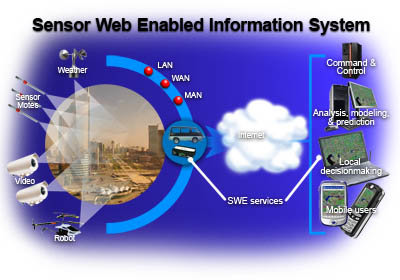
\includegraphics[width=0.6\textwidth]{figures/webswe.png}
 \caption{SWE architecture\label{fig:webswe}}
 \end{figure}
 
 
 The other challenge is to use a sensor's data for multiple purposes. For example a CCTV camera picture can be used to count the number of cars on the road, to get an estimation of the speedings in a crossing or to get visual weather data. Computer Vision algorithms, regressions and special machine learning algorithms need different computing resources. Those can be outsourced to different computers which must have access to the data. The Sensor Observation Server is used to make this all available.
 
 \section{Types of sensors}
 
 Sensors are all around us. We have sensors in our cell phones or any handheld devices. Most of them are connected to the Internet or a network. The measurements of all of these devices can be stored and queried from a database. The usable data in some devices are:
 
 \begin{itemize}
 	\item Smartphone
 	 \begin{itemize}
	 	 \item Camera: Visual image of the phone itself
	 	 \item Accelerometer: measurement of the acceleration of a system. Derivate of speed.
	 	 \item Weather sensors: Often smartphones has built in temperature sensors, rarely barometer is also installed.
	 	 \item Computing resource: ability to run additional softwares by using up its resources
	 	 \item Gyroscope: Orientation sensor.
 	 \end{itemize}
 	 \item Weather sensor
 	 \begin{itemize}
 	 \item Temperature sensor: Inner and outer temperature.
 	 \item Humidity sensor: percentage of humidity.
 	 \item Barometer: Air pressure.
 	 \end{itemize}
 	 \item Beagleboard
 	 \begin{itemize}
	\item Computing resource.
 	 \end{itemize}
 \end{itemize}

The examples show that a standard way to retrieve the measurements should include not only the measurement, but the type of the sensor, the measured unit, the location of the sensor and many additional information like this. 

Storing and retrieving this information is done using the SensorML format.

\section{The SensorML}

The Open Geospatial Consortium approved the SensorML language to be able to describe all the necessary information about measured data\cite{sensorml}. This is an XML based language that is used to describe the sensors, add, update, delete or retrieve information. The SensorML is able to solve the above mentioned problems. It is an abstract definition of the sensor information.

To have a general structure for the data, there is an abstract hierarchy that represents sensors and measurements. They have their own concepts which is described in as follows \cite{g2d2}:
\begin{itemize}
\item FeatureOfInterest: additional constraints provided for the measurement, e.g. time or location of measurement.
\item ObservedProperty: what type of physical property is measured, e.g. speed, temperature.
\item Procedure: the virtual or real sensor itself that is providing the data.
\item Offering: the property itself that has been measured, e.g. wind speed, air humidity, traffic size. 
\item Result: the output of the procedure.
\end{itemize}

This way gives as enough abstraction to separate the measured properties, the physical properties, the actual sensors and the results from each other.

It is able to define the location of the sensor, the timestamp of the measurement and the sensor data itself, with many additional information. The data can be stored in SOS servers that can retrieve the measurements on different interfaces. There are additional other services\cite{g4d3} that are present to add demanded functionalities to the service. These other service models are SAS, SPS and WNS, which are introduced below and SOS will be covered in details.

\section{Sensor Alerting Service}
This service model takes care of the broadcast of the messages. The clients can subscribe to some special messages or alerts and they will be notified if such an event has occurred. SAS is some kind of event notification service.

\section{Sensos Planning Service}
 
 This service provides a standard interface for controlling sensors and simulations. The SPS service implements the following tasks:
 \begin{itemize}
\item Description of the Tasks.
\item Verification of the feasibility of the tasks.
\item Status check of the running tasks.
\item Update or modification of running tasks.
\item Removal of tasks.
\end{itemize}

\section{Web Notification Service}
This service connects users with the sensor informations. This model provides a standard interface for communication between clients and the service through HTTP, instant messaging, e-mail, SMS, phone or fax. 
 
 
\section{Server Observation Service}

Server Observation Servers store SensorML data and let others query, manipulate and add sensors to the database. These sensors can be derived sensors. Such derived sensors are called procedures. A procedure can be a traffic information based on the CCTV camera. An SOS server should be able to handle dependencies based on which procedure requires other procedures to provide data. Sometimes derived sensors are also called virtual sensors, because they don't do physical measurement but provide a derived value.

There are many closed and open source implementations of SOS servers. Some open source implementations are introduced here.

The \textbf{MapServer} is written in C, C++, however it can be extended in many other languages\cite{mapserver}. It has a built in GUI to view data, however it is not yet available for the SOS implementation. The server can only be reached by one interface. It was originally developed by University of Minnesota. In the time of writing the paper the code is maintained and supported by the Open Source Geospatial Foundation. It is mostly used for mapping not for serving data for derived sensors. It was used in some projects between NASA and the University of Minnesota. 

\textbf{istSOS} is another implementation in Python\cite{istsos}. It runs its scripts from Apache web server just like MapServer. It uses PostgreSQL database backend to store values. It has a nice GUI for administration. Only supports standard SensorML interface to retrieve data. It is a project of the SUPSI University in Switzerland.

\textbf{OOSThetys} is a basic toolkit for enabling SensorML communication. It is written in Perl and Java. It is fairly documentated and seems to be abandoned because there has been no new release since the February of 2012.

\textbf{52north SOS} is a sample implementation written in Java\cite{52north}. It runs as a web service from Apache tomcat to serve requests. It also uses PostgreSQL with PostGIS extension. The application is used in the sample implementation and it is covered in details later.

All SOS servers and the whole SensorML standard is missing the semantic information about the sensors meaning that all sensor data are stored in such a database and all properties can be described for the sensors but no connection between the concepts can be described for the sensor.

\section{52north SOS server}

This implementation is done by the non profit organization with the identical name. The software supports many interfaces to query the information needed. The standard SOAP can be used to work with Java Web services. There are KVP and POX to retrieve or add data using standard GET queries. A big advantage is that 52north SOS supports JSON interface. It enables JSON queries to retrieve information efficiently in JavaScript, PHP, Python or other modern scripting languages.

The new 4.2 version is easy to install, it has a graphical user interface to set up the database connection and initialize the database. PostgreSQL with PostGIS is required.  The basic usage is described on  52north webpage, but sample queries are shown in the built in test client. 

The project is built with Maven and uses Spring framework too. The included unit tests ensure that the software's architecture is still consistent after compilation. The project was chosen to be part of Google's Summer of Code 2014 and the project gained a lot improvements from that. 

A request can be sent using the connector of each interface. This used to be done by adding the interface name to the application url but in recent versions the service automatically detects the interface from the HTTP metadata. For example http://152.66.253.152:8080/52n-sos-webapp/service is the url where all interface can be reached. The first part is the host of the server. The tomcat application server is listening on port 8080. 52n-sos-webapp is the default name of the web application, service it the default connector for the webservice. The sent HTTP content-type header marks the interface. A detailed description of the interfaces can be seen on table \ref{tab:services}.
\begin{table}[h]
\begin{center}
\begin{tabular}{| l | l | p{8cm} |}
\hline
Interface  & Content type & Description \\ \hline \hline
SOAP & application/soap+xml & Standard SOAP request mostly used in JAVA, it is sending the request in XML format using POST request. \\ \hline
POX & application/xml & Very similar to SOAP but has a different XML format. \\ \hline
KVP & application/xml & This is a GET request, meaning that all request parameters are encoded in the URL. The answer is in XML format. \\ \hline
JSON & applicaton/json & This is a POST request which sends and receives information using JSON objects. Most programming languages can easily parse this type of request.\\ \hline
\end{tabular}
\caption{Interfaces for 52n SOS server\label{tab:services}}
\end{center}
\end{table}


\section{SOS commands}
There are many commands to query or manipulate the SOS server. In this section some of them will be shown using the JSON interface. 

The GetCapabilities command (shown on Listing \ref{lst:getcap}) allows the clients to retrieve a list of the reachable sensors of the server and their configuration. This command lists all the available measurements on the server too. This call does not have any required parameters, only if the details of the response should be controlled. Such detail is the section to be displayed. There are 4 different sections:
\begin{itemize}
\item ServiceIdentification: the list of profiles that the server has been using. These profiles describe the format that the data is represented in.
\item ServiceProvider: in this section is the contact information for the operator of the SOS service.
\item OperationMetadata: this section provides the available options and their possible values.
\item FilterCapabilities: what fields are available for filtering. Can be spatial filtering for location or temporal filtering for time range.
\item Contents: summary of the type and FOI of each procedure. 
\end{itemize}

\begin{lstlisting}[caption={JSON getCapabilities POST request\label{lst:getcap}}]
{
  "request": "GetCapabilities",
  "service": "SOS",
  "sections": [
    "ServiceIdentification",
    "ServiceProvider",
    "OperationsMetadata",
    "FilterCapabilities",
    "Contents"
  ]
}
\end{lstlisting}

 If the procedure is known the DescribeSensor command will describe the measurements of the selected sensor. The response will include a description field which contains the details about the sensor in the standard XML based SensorML format. The sample request code can be seen on Listing \ref{lst:descsens}.

\begin{lstlisting}[caption={JSON DescribeSensor POST request\label{lst:descsens}}]
{
  "request": "DescribeSensor",
  "service": "SOS",
  "version": "2.0.0",
  "procedure": "http://www.52north.org/test/procedure/1",
  "procedureDescriptionFormat": "http://www.opengis.net/sensorML/1.0.1"
}
\end{lstlisting}

After knowing the necessary parameters the getObservation property can be called. This command shows the measured values for some given observations. The input can be complex, it can filter based on procedures, offerings, observed properties, on any feature of interest or temporal or spatial filters. A sample can be read from Listing \ref{lst:getobs}.

\begin{lstlisting}[caption={JSON GetObservation POST request with all filters\label{lst:getobs}}]
{
  "request": "GetObservation",
  "service": "SOS",
  "version": "2.0.0",
  "procedure": [
    "http://www.52north.org/test/procedure/6",
    "http://www.52north.org/test/procedure/1"
  ],
  "offering": [
    "http://www.52north.org/test/offering/6",
    "http://www.52north.org/test/offering/1"
  ],
  "observedProperty": [
    "http://www.52north.org/test/observableProperty/1",
    "http://www.52north.org/test/observableProperty/6"
  ],
  "featureOfInterest": [
    "http://www.52north.org/test/featureOfInterest/6",
    "http://www.52north.org/test/featureOfInterest/1"
  ],
  "spatialFilter": {
    "bbox": {
      "ref": "om:featureOfInterest/sams:SF_SpatialSamplingFeature/sams:shape",
      "value": {
        "type": "Polygon",
        "coordinates": [
          [ [ 50, 7 ],
            [ 53, 7 ],
            [ 53, 10],
            [ 50, 10],
            [ 50, 7 ]
          ]
        ]
      }
    }
  },
  "temporalFilter": [
    {
      "during": {
        "ref": "om:phenomenonTime",
        "value": [
          "2012-11-19T14:00:00+01:00",
          "2012-11-19T14:05:00+01:00"
        ]
      }
    },
    { 
      "equals": {
        "ref": "om:phenomenonTime",
        "value": "2012-11-19T14:08:00+01:00"
      }
    }
  ]
}
\end{lstlisting}

The response (on Listing \ref{lst:sendobs}) will contain the usual header which is contained by all the responses. It tells the requester the version of the response. After that comes the list of the observations that fit the conditions given. In the observation objects there are the procedures that measured the result, the feature of interests and the observable property that has been measured. The result object contains the uom field which is an abbreviation for the unit of measurement and the specific value. It can be an integer value, floating point or some encoded binary data.

\begin{lstlisting}[caption={JSON GetObservation response\label{lst:sendobs}}]
{
    "request": "GetObservation",
    "version": "2.0.0",
    "service": "SOS",
    "observations": [
        {
            "type": "http://www.og.net/def/observationType/OGC-OM/2.0/OM_Measurement",
            "procedure": "http://www.52north.org/test/procedure/6",
            "offering": "http://www.52north.org/test/offering/6",
            "observableProperty": "http://www.52north.org/test/observableProperty/6",
            "featureOfInterest": {
                "identifier": {
                    "codespace": "http://www.opengis.net/def/nil/OGC/0/unknown",
                    "value": "http://www.52north.org/test/featureOfInterest/6"
                },
                "sampledFeature": "http://www.52north.org/test/featureOfInterest/world",
                "geometry": {
                    "type": "Point",
                    "coordinates": [
                        51.447722,
                        7.270806
                    ]
                }
            },
            "phenomenonTime": "2012-11-19T13:09:00.000Z",
            "resultTime": "2012-11-19T13:09:00.000Z",
            "result": {
                "uom": "test_unit_6",
                "value": 2.9
            }
        },
        {
            "type": "http://www.og.net/def/observationType/OGC-OM/2.0/OM_Measurement",
            "procedure": "http://www.52north.org/test/procedure/6",
            "offering": "http://www.52north.org/test/offering/6",
            "observableProperty": "http://www.52north.org/test/observableProperty/6",
            "featureOfInterest": {
                "identifier": {
                    "codespace": "http://www.opengis.net/def/nil/OGC/0/unknown",
                    "value": "http://www.52north.org/test/featureOfInterest/6"
                },
                "sampledFeature": "http://www.52north.org/test/featureOfInterest/world",
                "geometry": {
                    "type": "Point",
                    "coordinates": [
                        51.447722,
                        7.270806
                    ]
                }
            },
            "phenomenonTime": "2012-11-19T13:03:00.000Z",
            "resultTime": "2012-11-19T13:03:00.000Z",
            "result": {
                "uom": "test_unit_6",
                "value": 2.3
            }
        }
    ]
}
\end{lstlisting}

If only the result fields are important to the user the shorter GetResult command can be used. It is shown on Figure \ref{lst:getresult}.

\begin{lstlisting}[caption={JSON minimal GetResult POST request\label{lst:getresult}}]

{
  "request": "GetResult",
  "service": "SOS",
  "version": "2.0.0",
  "offering": "http://www.52north.org/test/offering/6",
  "observedProperty": "http://www.52north.org/test/observableProperty/6"
}
\end{lstlisting}

The response will be a list of values of the last measurement for the queried properties. The results will be given as a concatenated string where each measurement is separated by a comma and in each measurement the value and its timestamp is separated by a hash mark. It can be seen on Figure \ref{lst:sendresult}.

\begin{lstlisting}[caption={JSON GetResult response\label{lst:sendresult}}]
{
    "request": "GetResult",
    "version": "2.0.0",
    "service": "SOS",
    "resultValues": "10#2012-11-19T13:00:00.000Z,2012-11-19T13:00:00.000Z,
    2.0#2012-11-19T13:01:00.000Z,2012-11-19T13:01:00.000Z,
    2.1#2012-11-19T13:02:00.000Z,2012-11-19T13:02:00.000Z,
    2.2#2012-11-19T13:03:00.000Z,2012-11-19T13:03:00.000Z,
    2.3#2012-11-19T13:04:00.000Z,2012-11-19T13:04:00.000Z,
    2.4#2012-11-19T13:05:00.000Z,2012-11-19T13:05:00.000Z,
    2.5#2012-11-19T13:06:00.000Z,2012-11-19T13:06:00.000Z,
    2.6#2012-11-19T13:07:00.000Z,2012-11-19T13:07:00.000Z,
    2.7#2012-11-19T13:08:00.000Z,2012-11-19T13:08:00.000Z,
    2.8#2012-11-19T13:09:00.000Z,2012-11-19T13:09:00.000Z,
    2.9"
}
\end{lstlisting}

There are other commands that manipulate the database, like InsertSensor, DeleteSensor to add or remove sensors. There are commands to add observable properties, and add results to the database too. 

Client applications use these services to communicate with the servers. These applications show the user a user friendly interface to read the measured data or their locations on a map. Such systems are described in the following sections.

\section{SOS client applications}

As the format introduced before is hard to decode for human there are various tools to display stored data in a user friendly way. With these tools measurements can be plotted in time, compared with each other and sensor locations can be displayed using a map. Even measurements can be plotted to a map giving a nice visual aid for processing the measured data. 

52north has an official client application for the SOS server called 52n Sensorweb Client. This is a Java web application that can be configured to connect to multiple hosts and display their sensor data on maps and charts. It is developed using the same tools as the SOS server. 
This means that the application can be installed next to the SOS server without any extra needs. This client can be opened in a web browser, but some parts run on the backend. This is a relatively complex application that does not yet understand semantic connections between the procedures. A screenshot can be seen on Figure \ref{fig:sweclient}.

\begin{figure}[h]
\centering
%http://sensorweb.forum.52north.org/SWE-Client-Could-not-get-procedure-details-url-caused-by-java-lang-NullPointerException-td4025524.html
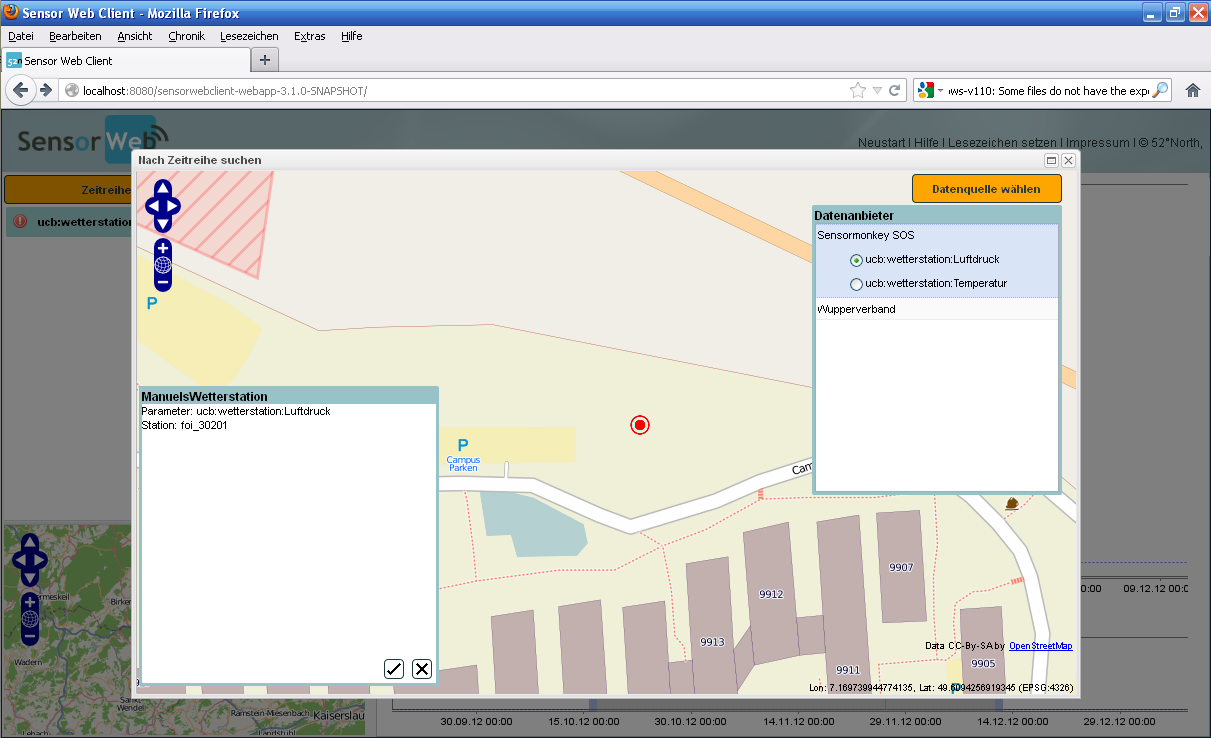
\includegraphics[width=0.6\textwidth]{figures/sweclient.png}
\caption{Screenshot of SWE Client 3\label{fig:sweclient}}
\end{figure}

There is a JavaScript framework that enables users to use only client side tools to connect to SOS servers and display data called SOS.js. Unfortunately, because of security restrictions on JavaScript cross-site request the data cannot be retrieved from the SOS server directly, the client has to be served from the same domain as the server. This is often not doable. That is why this application needs a proxy that forwards the data to the same domain to bypass this restriction. If the proxy is working, the framework can display everything just using the browser. Screenshot can be seen on Figure \ref{fig:sos-js}.

\begin{figure}[h]
\centering
%http://blog.52north.org/2014/02/21/sos-js/
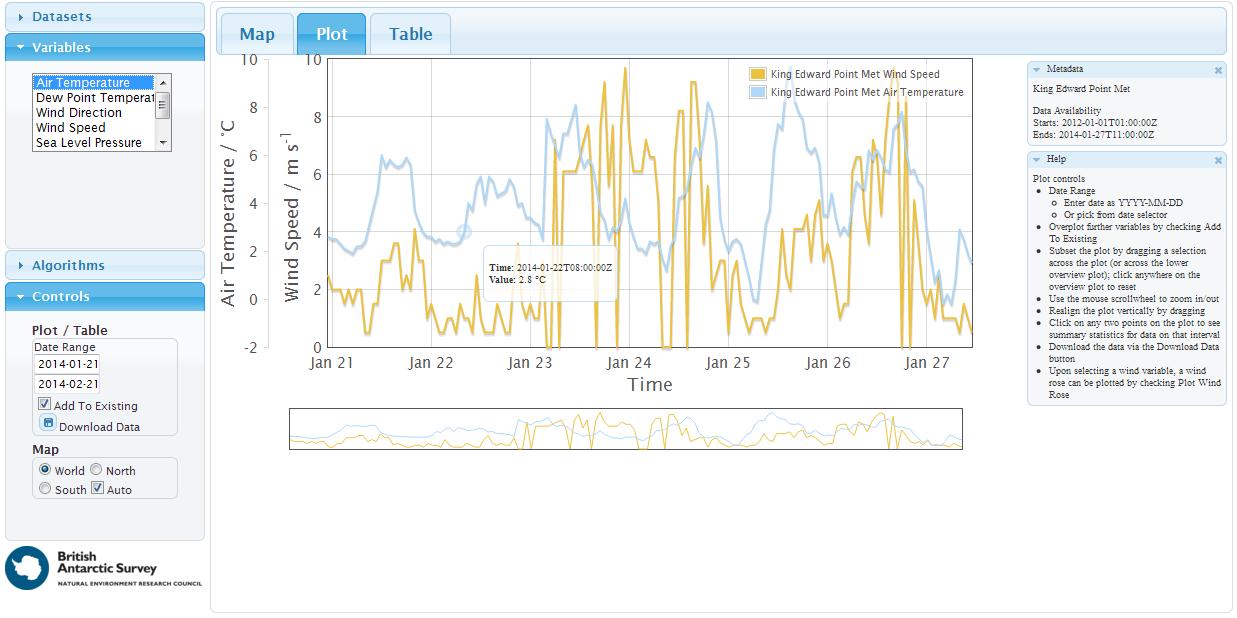
\includegraphics[width=0.6\textwidth]{figures/sos-js.png}
\caption{Screenshot of sos.js\label{fig:sos-js}}
\end{figure}

There are external softwares that can display their own measurements but not the SensorML standard. To make them usable with 52north SOS the developers created tools to extend such existing softwares to be able to import data from SOS.
Such extension is the ArcGIS extension which makes SOS data available to ArcGIS server. This is also available to other programs such as $\mu$Dig. 

There are other tools to export data to R language which is used to process large dataset for scientific purposes or to use with other Geographic Information Systems (GIS) softwares. However, the problem is that no client software has the ability to make search available by semantic connections. A client has to be extended with such information to enable convenient filtering when monitoring a cyberphisical system.

Fortunately there are standards to describe such systems and convert knowledge from one way to the other. This is described in the next chapter.
